\chapter{Evaluation}\label{sec:evaluation}
\todo[inline]{How and what can we evaluate?}
\todo[inline]{The performance?}
\todo[inline]{The flexibility?}

\section{Use case}\label{sec:use-case}
\todo[inline]{No section without text}

\subsection{Data Sets}
For our uses cases, we have two different data sets:
One data set consists of a user ranking of public broadcasting in Germany, i.e.\ entities, mostly TV and radio broadcasts, are liked or disliked by people.
This data is public data and can be used by media researchers of broadcasting corporations but also targets media journalists and the general audience.
The other set, called \riso{}, consists of statistical data from various German administrations and is used by the authorities for urban planning and policy strategies.

Both data sets share some characteristics.
The administrative data connects certain features with certain regions of Germany.
As Germany is a federal state, larger regions consist of many other smaller regions.

The second one consists of user data that was collected through a web application called \rufu{}.

\subsubsection{RISO}

The \riso{} data base is used in by local authorities to get insights about governmental KPIs to assist local and regional decision making.
It is a relational database and a part of the data base schema is shown as an ER diagram in Figure~\ref{fig:data:riso}.

\begin{figure}[h!]
  \centering
  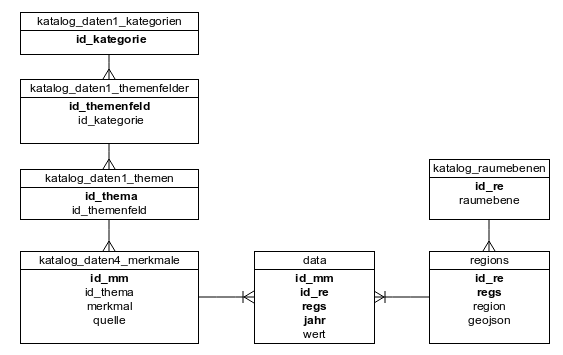
\includegraphics[width=\textwidth]{images/riso}
  \caption{Part of the \riso{} database schema. Primary keys are set in bold.}\label{fig:data:riso}
\end{figure}

The largest table is called \attr{data} with approximately 10,466,600 records, which holds all values along with the survey date.
\textbf{Features}
This data is connected to a feature table through a foreign key called \attr{id_mm}.
In the feature table we can find the description for every referenced feature, e.g.\ population density, working population in agriculture, education spending.
The \riso{} system groups all features in a 4-level hierarchy:
\begin{enumerate}
  \item
    \attr{katalog_daten_1_kategorien}
  \item
    \attr{katalog_daten_2_themenfelder}
  \item
    \attr{katalog_daten_3_themen}
  \item
    \attr{katalog_daten_4_merkmale}
\end{enumerate}
The actual features table is the last one in the list.
At the lowest level within the hierarchy, this is the largest table with 1234 records.


\textbf{Regions}
On the other side, the geographical data is stored in the \attr{regions} table.
The geometry data for each region is stored in the \attr{geojson} column and as the name suggests, the data type is a \attr{geojson}.
The foreign keys that connect the tables \attr{data} and \attr{regions} are called \attr{id_re} and \attr{regs}.
Unlike the feature table, the regions are grouped through the \attr{id_re} that indicates the hierarchy level.
So the values of the \attr{id_re} column denominate the level of the hierarchy.
E.g.\ a region with a \attr{id_re} of $1$ is a federal state of Germany, a region with id $13$ is a constituency.
A textual description for the hierarchy level can be found in the \attr{katalog_raumebenen} table in column \attr{raumebene}.
Both column \attr{id_re} and \attr{regs} belong to the primary key of the regions table, so there will never be two regions on the same hierarchy level with the same \attr{regs} id.

\textbf{Characteristics}
As we can see, the schema of the \riso{} database follows a rather denormalized approach.
The schema does not make a lot of assumptions regarding the input data.
It allows to add data of arbitrary size, features and completeness as long as there is some kind of numerical data associated with some kind of geographical unit.
This approach is suitable for a data base that incorporates data from different sources, as it is the case with the \riso{} data base.


\subsubsection{\rufu{}}
Unlike the \riso{} database, the data base of \rufu{} is used as persistence layer.
For that reason the data base schema follows the requirements of a web application in production.

As outlined in Section~\ref{sec:outline} \rufu{} is an evaluation platform for public broadcasting in Germany.
First, users vote on broadcasts, i.e.\ they decide if they want to support broadcast or if they do not want to support.
As a next step, user can define a weighting by distributing a virtual, monthly budget among the chosen broadcasts.

Figure~\ref{fig:data:rundfunk} shows the data base schema of the application.
A \attr{user} is connected to \attr{broadcast} through a \attr{selection}.
If the \attr{user} supports some a broadcast, the \attr{response} on the given \attr{selection} will be `positive'.
If the \attr{user} does not wish to support a \attr{broadcast}, the \attr{response} will be `neutral'.
The \attr{user} can allocate virtual money to supported broadcasts.
The money will be stored in the column \attr{amount} of the \attr{selection}.
The sum of all amounts for one user will never exceed the virtual budget of 17.50€.

\begin{figure}[h!]
  \centering
  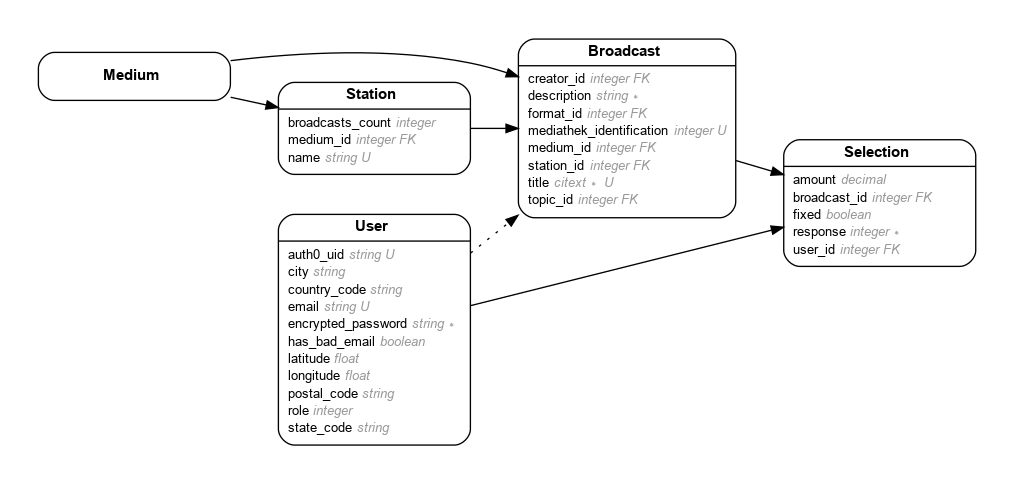
\includegraphics[width=\textwidth]{images/er}
  \caption{Database schema of the \rufu{} application}\label{fig:data:rundfunk}
\end{figure}

\textbf{Features}
We have both numerical as well as nominal features.
A numerical feature could be the number of supporters from an area in Germany.
A nominal feature could be a list of the most supported broadcasts from an area in Germany.
Numerical and nominal features can be combined, so we could request for every region, a distribution of the desired expenditure for radio, TV, online and other broadcasts.

\textbf{Regions}
\rufu{} stores the geometry for each region in \attr{geojson} files.
These files hold a \attr{FeatureCollection}.
Every \attr{Feature} is a region, the identifier is stored as a property.
We merge the geometry data with features for every request.
To be precise: We get all the user data, group it by the identifier \attr{state_code} and merge it with the geometry in the \attr{geojson}.

\textbf{Characteristics}
The data base schema is a result of the specific requirements of the persistence layer.
Changes in the source code may require a migration of the data base schema.

However, we can ask a lot of questions already with common data base queries or standard data analysis tools:
\begin{enumerate}
  \item
    How does the actual support of a broadcast compare to the average support of a broadcast?
  \item
    What are the most popular broadcasts in Berlin?
  \item
    What is the desired ratio of genres of supported broadcasts? How important is education compared to sport?
  \item
    How does the support of a broadcast change over time?
  \item
    According to the user ranking, which broadcasts are similar to each other?
\end{enumerate}


\section{Existing Interactions}
We will now classify the implemented interactions of our two applications according to the classification by \textcite{Yi2007} in Section~\ref{sec:interaction-theory:categories}.

\textbf{In our \visan{}} possible interactions can be categorized into the classes \emph{select}, \emph{explore}, \emph{reconfigure}, \emph{encode} and \emph{filter}.
As seen in Figure~\ref{fig:analysis:interaction:existing} the user can \emph{select} one item in the view by clicking on it.
The user can reveal a tooltip showing the item properties by hovering with the mouse on the item, which is another \emph{selection}.
The user can \emph{explore} the map in the usual manner:
If the user drags with the mouse on the map, a panning operation is performed with the viewpoint focused on Germany, i.e.\ the camera moves around like a turntable.
The zoom factor can be changed by scrolling on the canvas of the map.
\emph{Encode} and \emph{reconfigure} techniques are performed through the menu on the left side:
Under the ``features'' tab, the user can \emph{reconfigure} different data sets and the displayed diagram, e.g.\ a tree map visualization based on the geometry shape, cubes or voronoi regions.
The tab ``Dimensions'' allows the user to \emph{encode} properties of a data set to visual attributes, e.g.\ the height, color and texture of an item.
The tab ``Filter'' can be used to reduce the displayed data set along a range of continuous values.
Figure~\ref{fig:analysis:interaction:existing:filter} shows the range of visible values in the left menu.
When the user drags the slider, the items in the map on the right side are updated interactively.

\begin{figure}[h!]
  \centering
  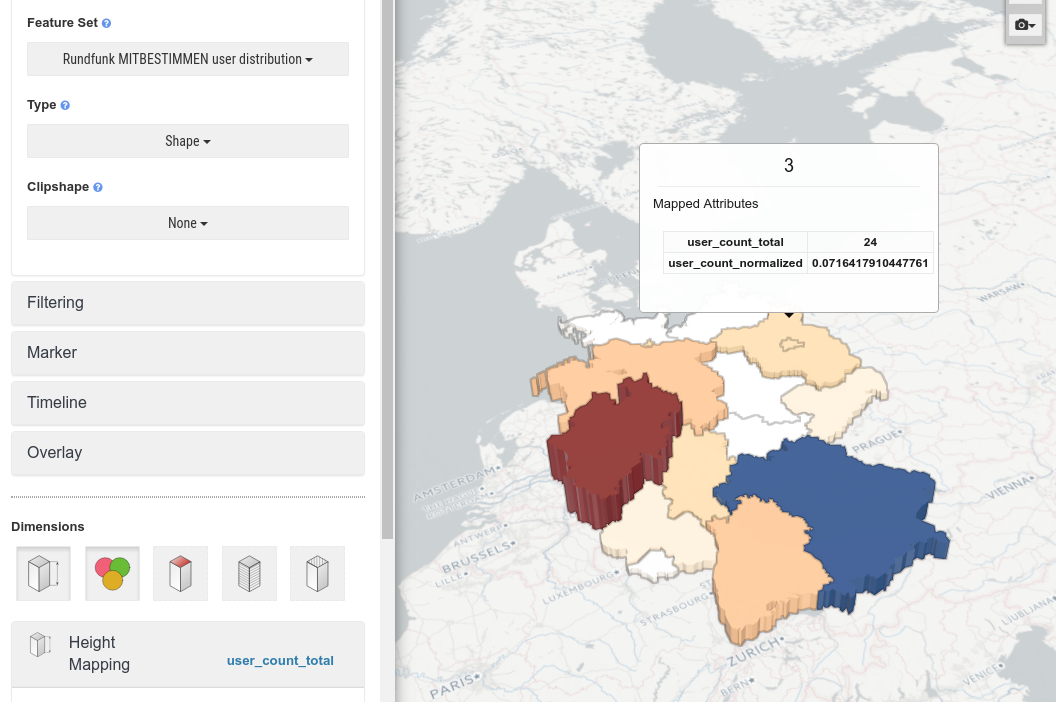
\includegraphics[width=\textwidth]{images/existing-interactions.png}
  \caption{%
    Items can be highlighted with a click, Bavaria is currently highlighted.
    A mouse over reveals a tooltip showing item properties.
    The menu on the left side allows to change the data set and the specific base visualization.
  }\label{fig:analysis:interaction:existing}
\end{figure}

\begin{figure}[h!]
  \centering
  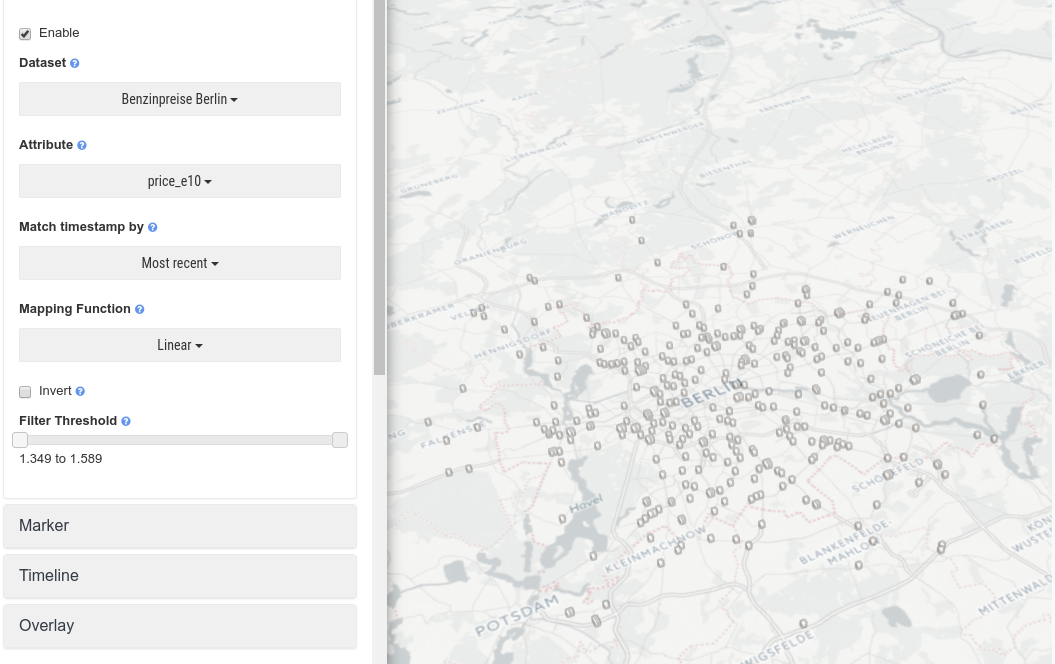
\includegraphics[width=\textwidth]{images/existing-interactions-filter.png}
  \caption{%
    Only gas stations with a price for E10 within 1.349 Euro and 1.589 Euro are displayed in the map
  }\label{fig:analysis:interaction:existing:filter}
\end{figure}

\section{Planned Interactions}
We have a focus on coordinated multiple views consisting of a tree map and a geographical map.
Let's have some examples how an interaction between a \tmap{} and a \map{} might work:

    \begin{enumerate}
      \item
        User selects a feature set from the drop down in the menu. This will trigger a \emph{Reconfigure} interaction. A data set consisting of all features and their ids, geometries and metadata is transferred. The receiving components are both the \tmap{} and the \map{} which will rerender the entire visualization.
      \item
        User hovers with a mouse over a polygon in the \map{}. This will trigger a \emph{Select} interaction. The data is a single feature id that will be transferred to the \tmap{}, which will change the color of an box.
      \item
        Rotate or zoom the \tmap{}. This will also rotate or zoom the \map{}. The interaction would fall into \emph{Explore} and the shared information is the orientation of the camera and the zoom level.
      \item
        A click in the \tmap{} will trigger an \emph{Explore} interaction. The data is a single feature id sent to the \map{}. The map will center the viewport on the center of geometry of the respective feature.
      \item
        The user selects many features at once in the \map{} by dragging a rectangle. The ids of all features within the rectangle are sent to the \tmap{}. All features will be highlighted with a different color, which is therefore a \emph{Select} interaction.
      \item
        \emph{Reconfigure} the layouting of the \tmap{} by choosing a different hierarchy level. This increased granularity may lead to an increased granularity in the \map{}, e.g.\ show postal codes instead of federal states. The changed data are additional items, that are nested in the former items.
      \item
        \emph{Encode} the \tmap{} by a different attribute mapping like color, height or texture. If the \map{} has no geometry data that defines the shape of a feature, it can also display a larger point marker.
      \item
        Apply a \emph{Filter} and reduce the data set by choosing only items with metadata beyond a certain treshold. The reduced data leads to a full re-render of all data visualizations. The message contains the updated item list
  \item
    Show a \emph{Connect} by highlighting boxes of the same subtree in the \tmap{}. The respective connected items would be highlighted in the \map{} as well. Here the data is a relation between items.
    \end{enumerate}
\todo[inline]{What are the key interactions in our use case?}

